% Latex template: https://github.com/mqTeXUsers/Macquarie-University-Beamer-Theme

% Slide Masters:

% Title
% Text
% 2 column
% Full-image
% Bibliography
% Closing
 
\documentclass[aspectratio=169, 12pt]{beamer} % Aspect ratio
% https://tex.stackexchange.com/a/14339/5483 
% Possible values: 1610, 169, 149, 54, 43 and 32.
% 169 = 16:9

\PassOptionsToPackage{table}{xcolor}    %https://tex.stackexchange.com/a/5365/5483

\usetheme{macquarie}
\usepackage{multicol} % https://tex.stackexchange.com/a/396018/5483

\usepackage{svg} %https://github.com/mrpiggi/svg 

\usepackage[english]{babel}       % Set language
% \usepackage[utf8x]{inputenc}      % Set encoding
\usepackage{colortbl}
\mode<presentation>           % Set options
{
  \usetheme{default}          % Set theme
  \usecolortheme{default}         % Set colors
  \usefonttheme{default}          % Set font theme
  \setbeamertemplate{caption}[numbered] % Set caption to be numbered
}

% Uncomment this to have the outline at the beginning of each section highlighted.
%\AtBeginSection[]
%{
%  \begin{frame}{Outline}
%    \tableofcontents[currentsection]
%  \end{frame}
%}

\usepackage{graphicx}         % For including figures
\usepackage{booktabs}         % For table rules
\usepackage{hyperref}         % For cross-referencing


\usepackage{enumitem} % https://tex.stackexchange.com/a/2292/5483

%https://tex.stackexchange.com/a/371844/5483
\setbeamerfont{bibliography entry author}{size=\tiny}
\setbeamerfont{bibliography entry title}{size=\tiny}
\setbeamerfont{bibliography entry location}{size=\tiny}
\setbeamerfont{bibliography entry note}{size=\tiny}
\setbeamerfont{bibliography item}{size=\tiny}

%https://tex.stackexchange.com/q/333587/5483
%TODO SHAWN REPLACE OSF URL
%\setbeamertemplate{footline}{\strut~\texttt{https://osf.io/v5jp7/}\hfill\insertframenumber~/~\inserttotalframenumber\strut~~~}

\title{Seven years of FAIMS Mobile} % Presentation title
\author{Shawn A Ross}               % Presentation author
\institute{Office of the Deputy Vice-Chancellor (Research)}         % Author affiliation
\date{\today}                 % Today's date  
\begin{document}

% Title page
% This page includes the informations defined earlier including title, author/s, affiliation/s and the date
% \begin{frame}[noframenumbering]

\maketitle

  
% \end{frame}

% Outline
% This page includes the outline (Table of content) of the presentation. All sections and subsections will appear in the outline by default.
\begin{frame}{Strategies for field data capture infrastructure}
  \tableofcontents
\end{frame}

% The following is the most frequently used slide types in beamer
% The slide structure is as follows:
%
%\begin{frame}{<slide-title>}
% <content>
%\end{frame}

% Slides to speak to at CAA2019

% In-depth information for reference
\section{Transparency and reproducibility}

\begin{frame}{The `reproducibility crisis'}
  For nearly a decade the reproducibility crisis has featured in the scientific literature \cite{Jasny2011-bw, Baker2016-cf, Munafo2017-bj}. Low reproducibility rates have emerged from large-scale studies:
    \begin{itemize}[label=\textbullet]
        \item Results from only 39\% of psychology studies could be reproduced \cite{Open_Science_Collaboration2015-vf}.
        \item Even lower reproducibility rate in biomedical research \cite{Begley2012-xt,Prinz2011-za}.
    \end{itemize}
\end{frame}

\begin{frame}{Perceptions of the reproducibility crisis}
  \begin{figure}[H]
    \centering
        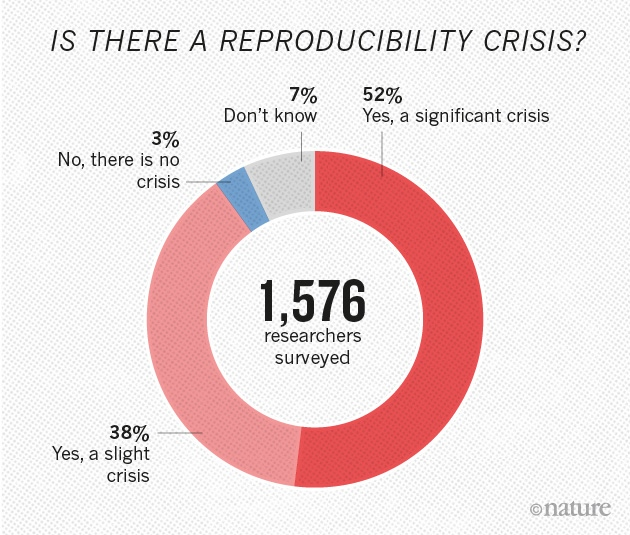
\includegraphics[height=.7\textheight]{figures/reproducibility-graphic-online1.jpeg}
        \caption{Is there a reproducibility crisis? \cite{Baker2016-cf}}
        \label{fig:figure3}
  \end{figure}
\end{frame}

\begin{frame}{Motivation: Preserving data}
 \begin{figure}[H]
    \centering
        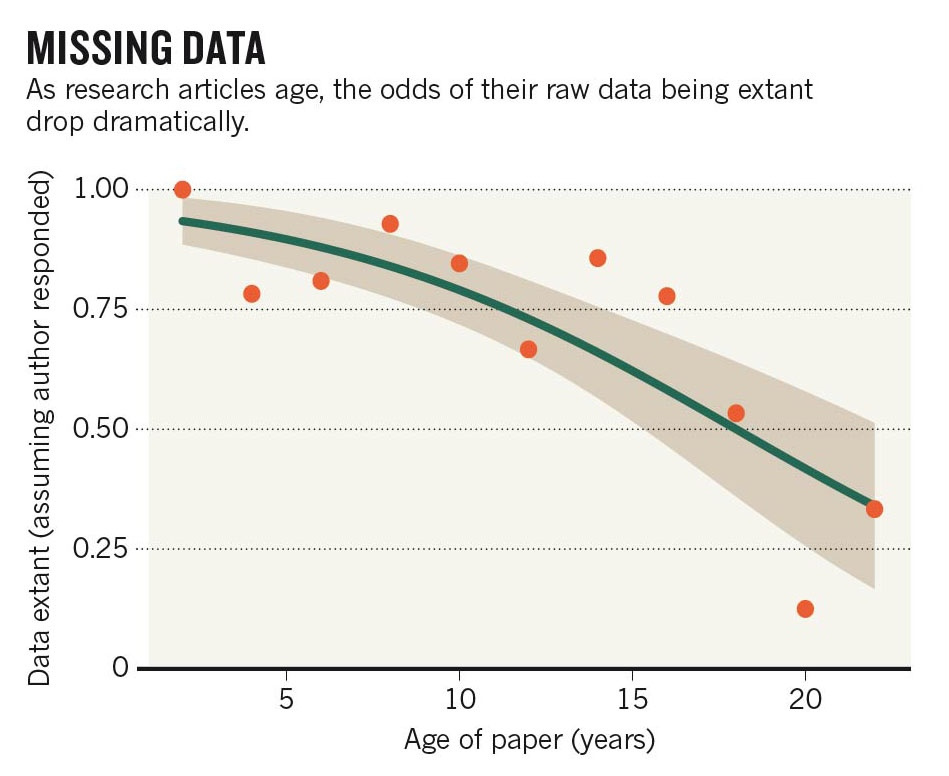
\includegraphics[height=.75\textheight]{figures/Missing-Data.png}
        \caption{\cite{Vines2014-zr}}
        \label{fig:vines2014}
 \end{figure}
\end{frame}

\begin{frame}{The response: improved rigour and transparency}
  Key guidelines to good practice:
    \begin{itemize}[label=\textbullet]
        \item Findable, Accessible, Interoperable, and Reusable (FAIR) data \cite{Wilkinson2016-mr, Go-fair2017-vs}.
        \item Transparency and Openness Promotion (TOP) guidelines \cite{Nosek2015-wm}.
        \item Data transparency toolkit \cite{Perkel2018-rw}.
    \end{itemize}
\end{frame}

\begin{frame}{The response: from guidelines to mandates}
  Mandates for transparency or reproducibility:
    \begin{itemize}[label=\textbullet]
        \item Nature: Transparency Upgrade \cite{Nature2017-lq}.
        \item Nature: FAIR data in Earth science \cite{Nature2019-ng}.
        \item Copernicus: FAIR data in atmospheric sciences \cite{Van_Edig2018-bu}.
        \item Not just the natural sciences: AJPS requires data and code \cite{Jacoby2017-lw, Ajps2015-ex}.
        \item TOP Guidelines signatories include publishers representing 1000+ journals, as well as professional organisations and major private foundations that fund research \cite{Cos2019-mr}.
        \item Funders' data policies \cite{Dcc2019-jn}
    \end{itemize}
\end{frame}


% https://tex.stackexchange.com/a/2292/5483
% https://ctan.org/pkg/enumitem?lang=en

\begin{frame}{Level 2 TOP Guidelines for authors (excerpt)}
  
    \begin{enumerate}[label=\arabic*.]
        \setcounter{enumi}{1}
        % This increments the enumerate counter by 1.
        
        \item Authors using original data must:
        \begin{enumerate}[label=\alph*.]

            \item make the data available at a trusted digital repository [...]
            \item include all variables, treatment conditions, and observations described in the manuscript.
            \item provide a full account of the procedures used to collect, preprocess, clean, or generate the data.
            \item provide program code, scripts, codebooks, and other documentation sufficient to precisely reproduce all published results.
            \item provide research materials and description of procedures necessary to conduct an independent replication of the research.
        \end{enumerate}
    \end{enumerate}
    \cite{Osf2014-pf}
\end{frame}

\begin{frame}{TOP Guidelines: publisher adoption}
  \begin{figure}[H]
    \centering
        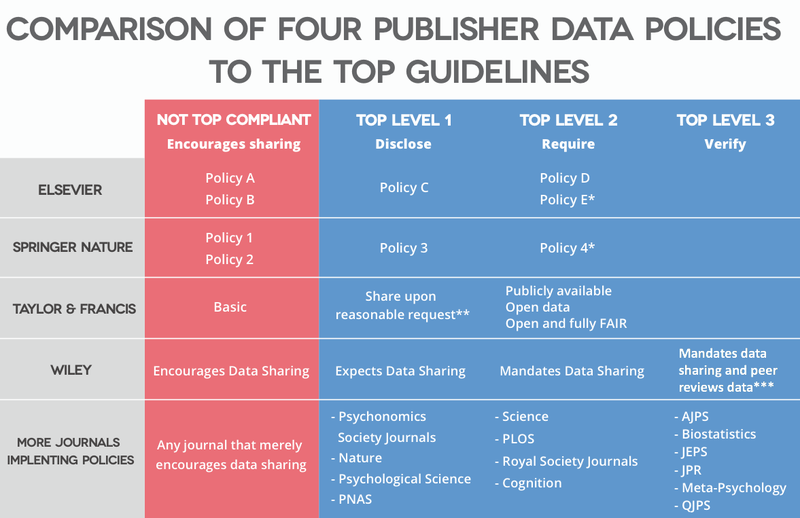
\includegraphics[height=.7\textheight]{figures/TOP-landscape.png}
        \caption{The Landscape of Open Data Policies \cite{Mellor2018-bf}}
        \label{fig:figure2}
  \end{figure}
\end{frame}

\begin{frame}{TOP Guidelines: funder endorsement}
  Private funders have endorsed via the Open Funders Research Group:
    \begin{itemize}[label=\textbullet]
        \item Alfred P. Sloan Foundation
        \item American Heart Association
        \item Bill and Melinda Gates Foundation
        \item Howard Hughes medical Institute
        \item John Templeton Foundation
        \item Laura and John Arnold Foundation
        \item Open Society Foundations
        \item Robert Wood Johnson Foundation
        \item Wellcome Trust
        \item and six more \cite{Ofrg2019-pq}
    \end{itemize}
\end{frame}

\begin{frame}{Other Funder data policies}
  \begin{figure}[H]
    \centering
        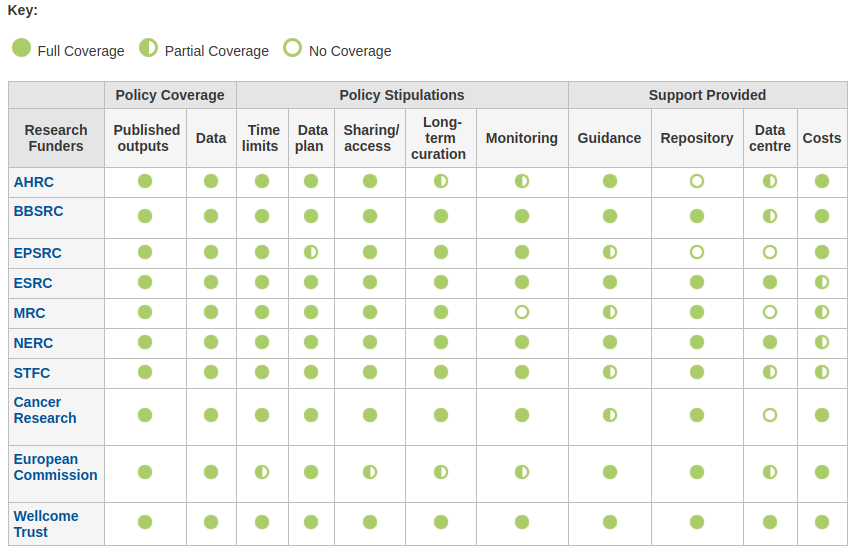
\includegraphics[height=.7\textheight]{figures/DCC-Funders.png}
        \caption{Overview of funders' data policies \cite{Dcc2019-jn}}
        \label{fig:Dcc2018}
  \end{figure}
\end{frame}

\begin{frame}{Data sharing in the NHMRC Statement}
    The NHMRC `strongly encourages' data sharing in the National Statement on Ethical Conduct in Human Research and their Open Access Policy. \cite{Nhmrc2018-sj, Nhmrc2018-vn} \par
    National Statement 3.1.50 \par
    In the absence of justifiable ethical reasons (such as respect for cultural ownership or unmanageable risks to the privacy of research participants) and to promote access to the benefits of research, researchers should collect and store data or information generated by research projects in such a way that they can be used in future research projects. Where a researcher believes there are valid reasons for not making data or information accessible, this must be justified.
\end{frame}

\begin{frame}{NHMRC Open Access Policy 2018 changes}
    Key changes to the Open Access Policy (15 January 2018) \par
    Research data and metadata (2.2) \par
    NHMRC now strongly encourages researchers to take reasonable steps to share research data and associated metadata arising from NHMRC supported research.\par
    FAIR principles (2.7) \par
    Reference to the Australian F.A.I.R. principles (Findable, Accessible, Interoperable, Reusable) when publishing research literature and sharing data has been made.
\end{frame}

\begin{frame}{NHMRC Open Access Policy data sharing}
    Medatdata (4.1) \par
    The metadata for the peer-reviewed publication must be made openly accessible via an institutional repository as soon as possible but no later than 3 months from the date of publication. \par
    Data (4.2) \par
    NHMRC acknowledges the importance of making research data publicly accessible and therefore strongly encourages researchers to consider the reuse value of their data and to take reasonable steps to share research data and associated metadata arising from NHMRC supported research.
\end{frame}

\begin{frame}{Legal compliance}
    \begin{itemize}[label=\textbullet]
        \item NSW General Retention and Disposal Authority GDA 23; data associated with `significant' research or researchers must be kept forever (23.6.1) \cite{Nsw2015-kv}
        \item NSW Privacy and Personal Information Protection Act 1998 No 133, esp. Part 2, Division 1, Section 19, which flags indicators of high sensitivity and establishes data sovereignty.\cite{Nsw1998-mw} Compare the (Australian) Privacy Act 1988, esp. Part II, Division 1, Section 6 `Sensitive Information' and Schedule 1, and `Australian Privacy Principles', Section 8, which covers some university-controlled entities. \cite{Ag2017-oz,Oaic2019-ng}
        \item NSW Notifiable Data Breach guidance \cite{Ipc_nsw2018-yr}; see also the Australian Notifiable Data Breaches scheme \cite{Oaic2019-dq}
        \item EU General Data Protection Regulation \cite{Gdpr2019-ee}
    \end{itemize}
\end{frame}

\begin{frame}{What does this mean? Are we ready?}
  Emerging good practice - and publisher and funder policies - mean:
    \begin{itemize}[label=\textbullet]
        \item Comprehensive, FAIR datasets will be deposited in domain-specific repositories. Data, and especially metadata, quality will be higher.
        \item Data will be captured digitally as early in research as possible, and provenance / version history maintained.
        \item Research approach, processes, and procedures will be documented.
        \item Data processing and analysis will use code (not Excel or ARCGIS!) 
        \item Code will be documented and published for reuse.
        \item Further steps taken for analytical reproducibility (use of OSS, version control, automation, containerisation, etc.). 
    \end{itemize}
\end{frame}

\begin{frame}{Beyond compliance: large-scale research}
    The same approaches that facilitate transparency and reproducibility support the kind of scalable and synthetic research that can address archaeological `grand challenges'. \cite{Kintigh2014-ub}
        \begin{itemize}[label=\textbullet]
            \item Paper data capture and manual digitisation and cleaning don't scale.
            \item Email and desktop software don't scale.
    \end{itemize}
\end{frame}

\begin{frame}{Scalable approaches to data and analysis}
  \begin{figure}[H]
    \centering
        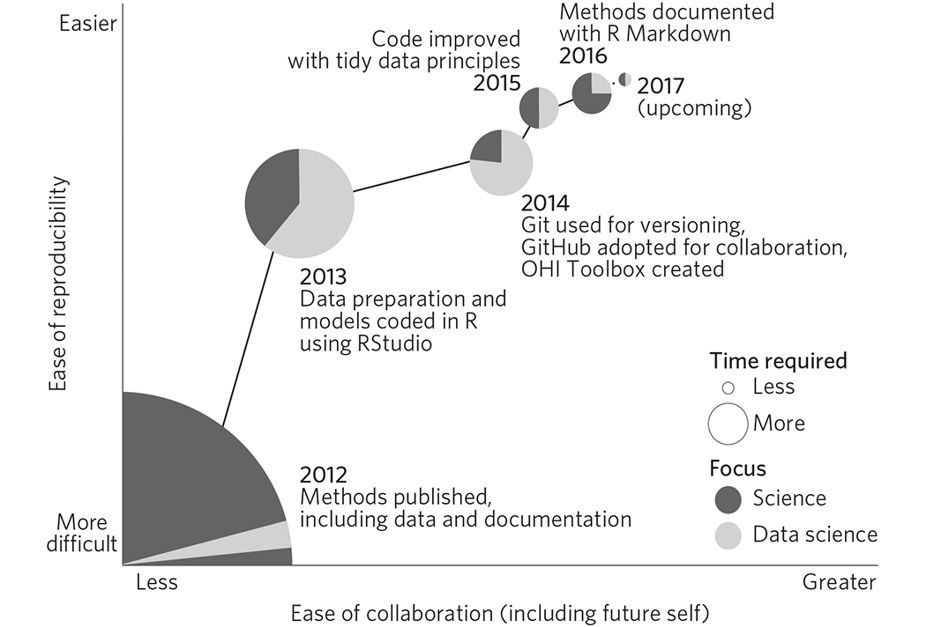
\includegraphics[height=.7\textheight]{figures/Ocean-Health-Index.jpg}
        \caption{Better science in less time, illustrated by the Ocean Health Index project. \cite{Stewart_Lowndes2017-lj}}
        \label{fig:figure14}
  \end{figure}
\end{frame}

\section{`Small data' infrastructure across the data lifecycle}

\begin{frame}{`Small data' research}
 \begin{figure}[H]
    \centering
        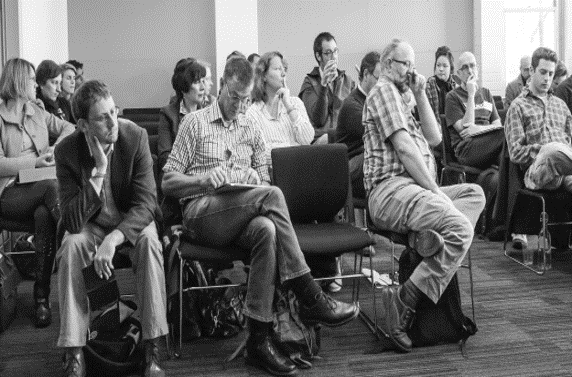
\includegraphics[height=.75\textheight]{figures/Archaeologists-standards.png}
        \caption{Archaeologists contemplate data standards (FAIMS Stocktaking, 2012)}
        \label{fig:figure7}
 \end{figure}
\end{frame}

\begin{frame}{Context: the challenge of `small data'}
    `Long tail' research: most field data is small data \cite{Borgman2015-rh}
    \begin{itemize}[label=\textbullet]
        \item Smaller scale; smaller communities; local control.
        \item Diverse questions, approaches, and methods.
        \item Heterogeneous data; variety of content, structure.
        \item Data and infrastructure emerge from fieldwork. 
        \item Relative lack of standards.
        \item Limited infrastructure and funding.
        \item Challenges associated with big(ger) data from photogrammetry, SfM, video, geophysics, etc., will exacerbate these problems.
    \end{itemize}
\end{frame}

\begin{frame}{The data lifecycle}
 \begin{figure}[H]
    \centering
        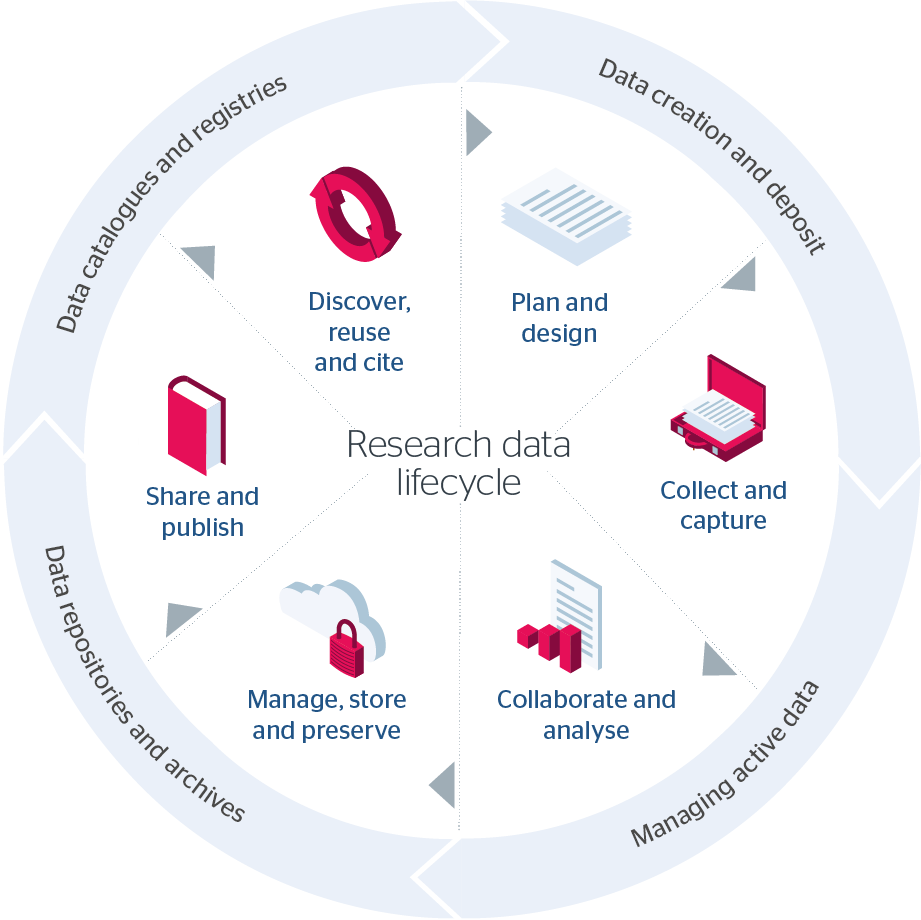
\includegraphics[height=.75\textheight]{figures/research-data-life-diagram.png}
        \caption{\cite{Jisc2018-gx} Image CC-BY-ND}
        \label{fig:figure9}
 \end{figure}
\end{frame}

\begin{frame}{Infrastructure across the data lifecycle}
    Consider the infrastructure needed to manage the three main phases of the data lifecycle
    \begin{itemize}[label=\textbullet]
        \item Publication (most mature): domain-specific repositories.
        \item Processing and analysis (less mature): project-level code \cite{Stewart_Lowndes2017-lj}, then Virtual Labs / Science Gateways, like \cite{Alveo2019-tk} in language analysis.
        \item Capture (least mature): most varied, needs to work offline under difficult conditions. Commercial solutions insufficient \cite{Bureau_of_Reclamation2017-xl}.
    \end{itemize}
\end{frame}


% Slides to speak to at WSU 5 June 2019

\section{Lessons from FAIMS: summary}

\begin{frame}{Research Specific}
 \begin{figure}[H]
    \centering
        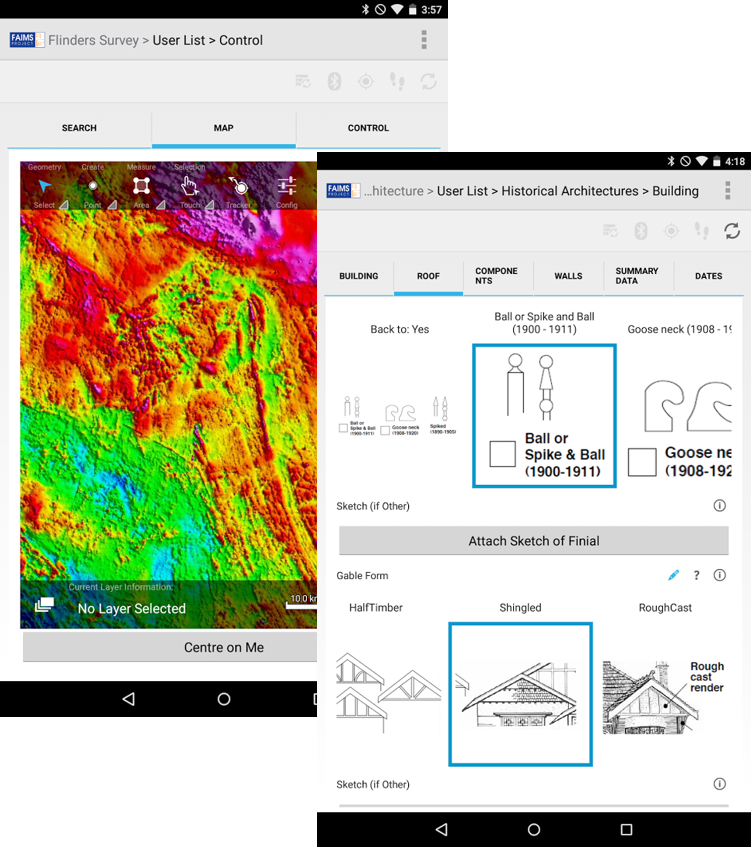
\includegraphics[height=.75\textheight]{figures/FAIMS-screenshots.png}
        \caption{FAIMS Mobile: GIS and `picture dictionaries'}
        \label{fig:FAIMS-mobile-screenshots}
 \end{figure}
\end{frame}


\begin{frame}{Generalised}
 \begin{figure}[H]
    \centering
        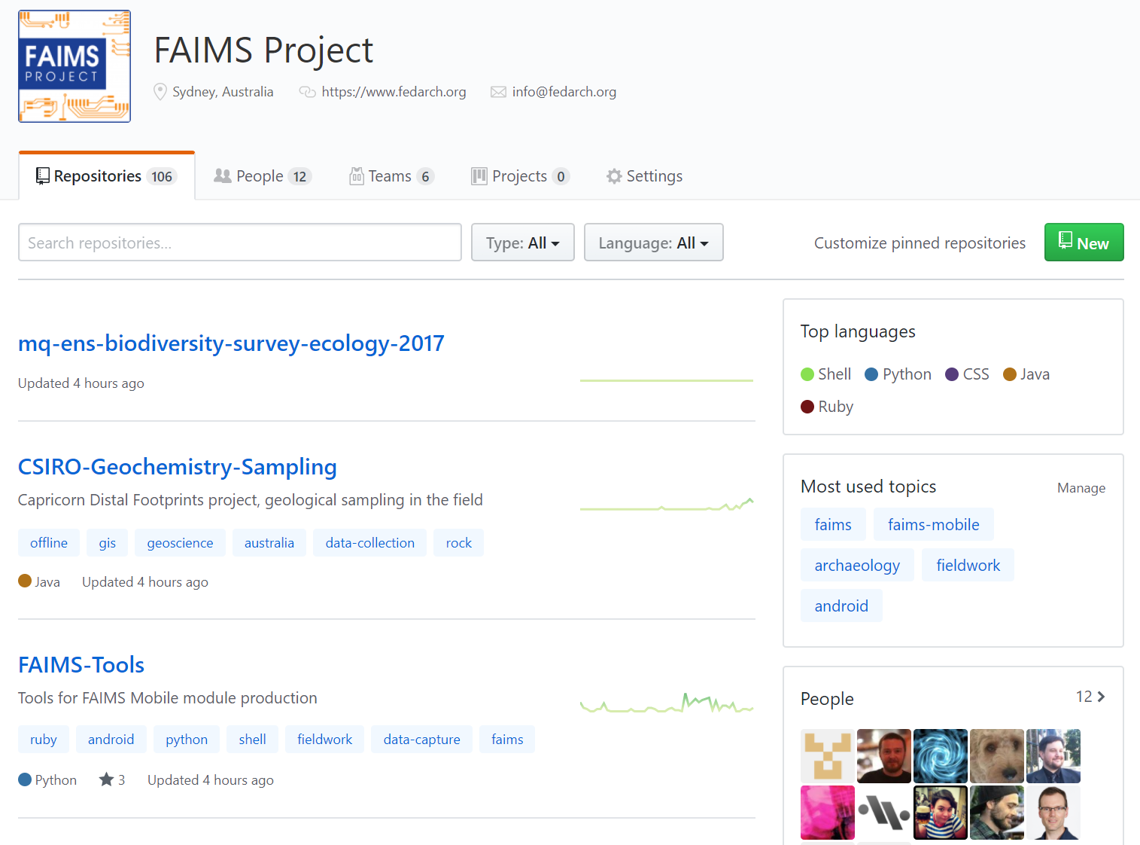
\includegraphics[height=.75\textheight]{figures/FAIMS-generalised.png}
        \caption{FAIMS Mobile customisations on GitHub}
        \label{fig:FAIMS-github}
 \end{figure}
\end{frame}

\begin{frame}{Modular and federated}
 \begin{figure}[H]
    \centering
        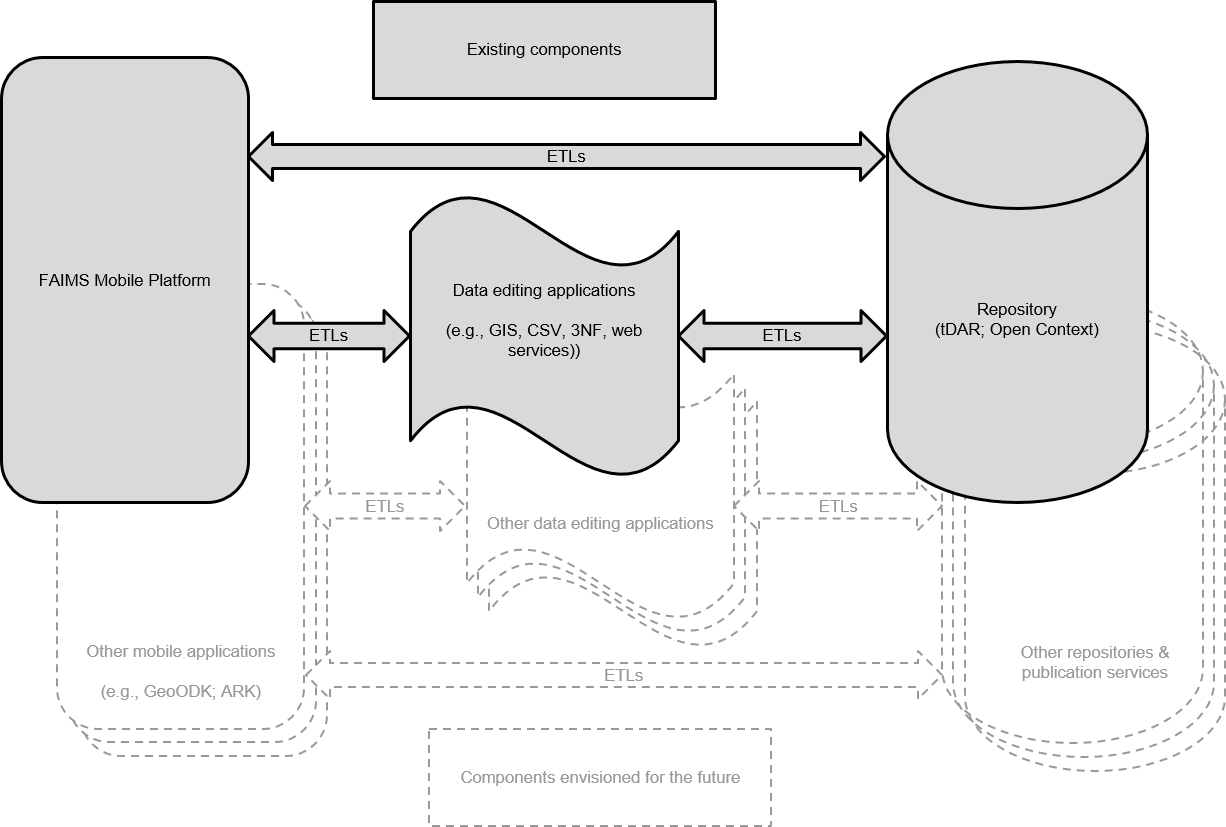
\includegraphics[height=.75\textheight]{figures/FAIMS-federated.png}
        \caption{FAIMS Mobile federation}
        \label{fig:FAIMS-federation}
 \end{figure}
\end{frame}

\begin{frame}{Open Source}
 \begin{figure}[H]
    \centering
        
\includegraphics[width=.75\textwidth]{figures/GPLv3_Logo.eps}
        \caption{FAIMS Mobile 'core' code is GPLv3}
        \label{fig:FAIMS-github-OSS}
 \end{figure}
\end{frame}

\begin{frame}{Small data collection infrastructure: key messages}
    \begin{itemize}[label=\textbullet]
        \item We deserve research-specific software.
        \item Diverse practices and limited resources require generalised software.
        \item Do one thing well with modular and federated software (but slice the pie thoughtfully).
        \item Open-source software has advantages (but is difficult to sustain). 
        \item Scope requirements carefully.
        \item Invest in outreach and engagement.
    \end{itemize}
\end{frame}

\begin{frame}{Challenges and paths forward}
  How do we get from where we are now to where we want to be?
      \begin{itemize}[label=\textbullet]
        \item Understand the evolving expectations of transparent research. 
        \item Look past desktop software (Excel, ARCGIS, Filemaker, Access, etc.).
        \item Rally around emerging research- and domain-specific solutions (even if imperfect).
        \item Overcome `not invented here'; you don't need a bespoke solution.
        \item Budget for `ground-up' transparency (data and code). Up-front costs will be high but offer longer-term payoffs (in costs, time, and quality).
        \item Implement (and budget for) fundamental good practice in data and code management before other technologies.
        \item Improve research design (prioritise approach over methods) \cite{Muthukrishna2019-kt, Hole1973-cy}
    \end{itemize}
\end{frame}

% In-depth information for reference
\section{Lessons from FAIMS: in-depth}

\begin{frame}{Introduction to the FAIMS Project}
    \begin{itemize}[label=\textbullet]
        \item The Field Acquired Information Management Systems (FAIMS) Project began in 2012 as a national Australian information infrastructure project in archaeology.
        \item Developed FAIMS Mobile for field data capture \cite{Ballsun-Stanton2018-zd}.
        \item Use expanded beyond archaeology to geoscience, ecology, ethnography, linguistics, oral history.
        \item Has been customised for over 50 workflows at more than 30 projects. 
        \item Data and workflow modelling for these customisations provided deep insights into field data capture and the infrastructure needed to support it.
    \end{itemize}
\end{frame}

\begin{frame}{FAIMS Mobile software}
 \begin{figure}[H]
    \centering
        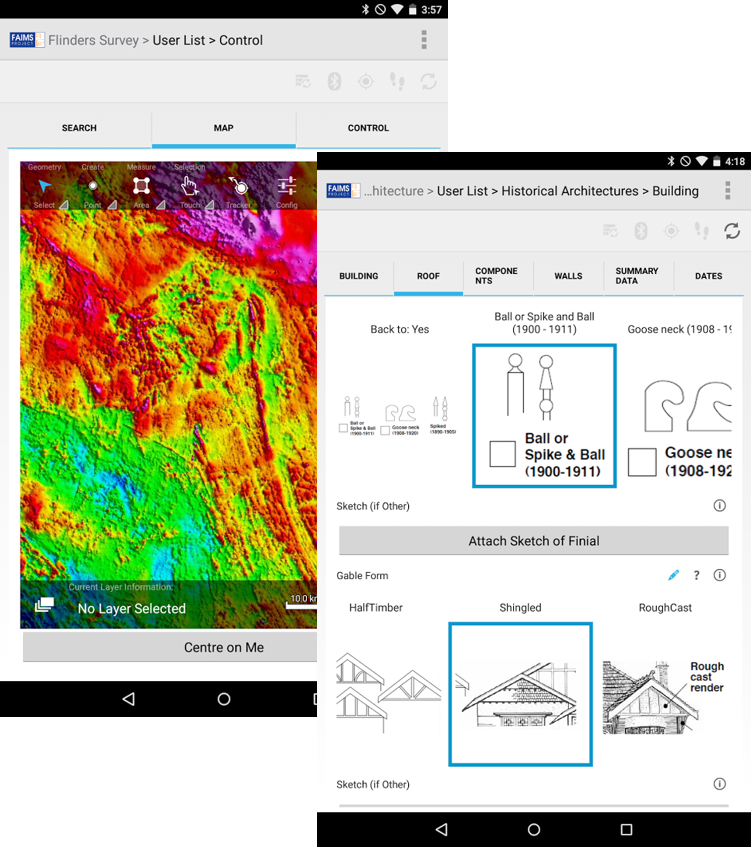
\includegraphics[height=.75\textheight]{figures/FAIMS-screenshots.png}
        \caption{FAIMS Mobile: GIS and `picture dictionaries'}
        \label{fig:figure10}
 \end{figure}
\end{frame}

\begin{frame}{Key research-specific FAIMS Mobile features}
    \begin{itemize}[label=\textbullet]
        \item Fundamentally customisable.
        \item Tightly binds structured, geospatial, multimedia, and free text data.
        \item Works offline.
        \item Automated bi-directional synchronisation using local or online server
        \item Record history: append-only datastore, versioning, rollback.
        \item Mobile GIS.
        \item Connects to internal and external sensors, Bluetooth / USB devices.
        \item Multilingual.
        \item Granular help.
        \item Granular metadata / uncertainty.
        \item Generalised export.
        \item `Hooks’ for data interoperability, Open Linked Data approaches.
    \end{itemize}
\end{frame}

\begin{frame}{Field data capture infrastructure: key messages}
    \begin{itemize}[label=\textbullet]
        \item We deserve research-specific software.
        \item Diverse practices and limited resources require generalised software.
        \item Do one thing well with modular and federated software (but slice the pie thoughtfully).
        \item Open-source software has advantages (but is difficult to sustain). 
        \item Scope requirements carefully.
        \item Invest in outreach and engagement.
    \end{itemize}
\end{frame}

\begin{frame}{Research specific}
    Archaeology needs (and deserves) research-specific software, contra \cite{Roosevelt2015-kd}.
      \begin{itemize}[label=\textbullet]
        \item Most commercial / mass-market software does not meet research needs.
        \item Risk of lock-in, unwelcome changes to features or business models, and product discontinuation.
    \end{itemize}
    Compare ecology in Australia: TERN, ALA, Biocollect, and associated research clouds \cite{Tern2019-sp, Ala2019-by, Ala2019-cb}.
\end{frame}

\begin{frame}{Generalised (not generic or bespoke)}
  Commercial software doesn't meet our needs, and bespoke development is too expensive and usually unsustainable.
      \begin{itemize}[label=\textbullet]
        \item Generalised software can be deeply customised to accommodate our diverse data types, data models, workflows, etc.
        \item The code used to customise it describes the data model and workflow.
        \item Customisations can be published and re-deployed trivially.
        \item Can deliver research-grade software affordably.  
    \end{itemize}
    FAIMS Mobile cost perhaps 3x a single bespoke application, but has been customised 50x. Customisation cost is 1/10th bespoke, and still <1/2 even if `core' platform development costs are amortised across projects.
\end{frame}

\begin{frame}{Generalised: customise using code}
 \begin{figure}[H]
    \centering
        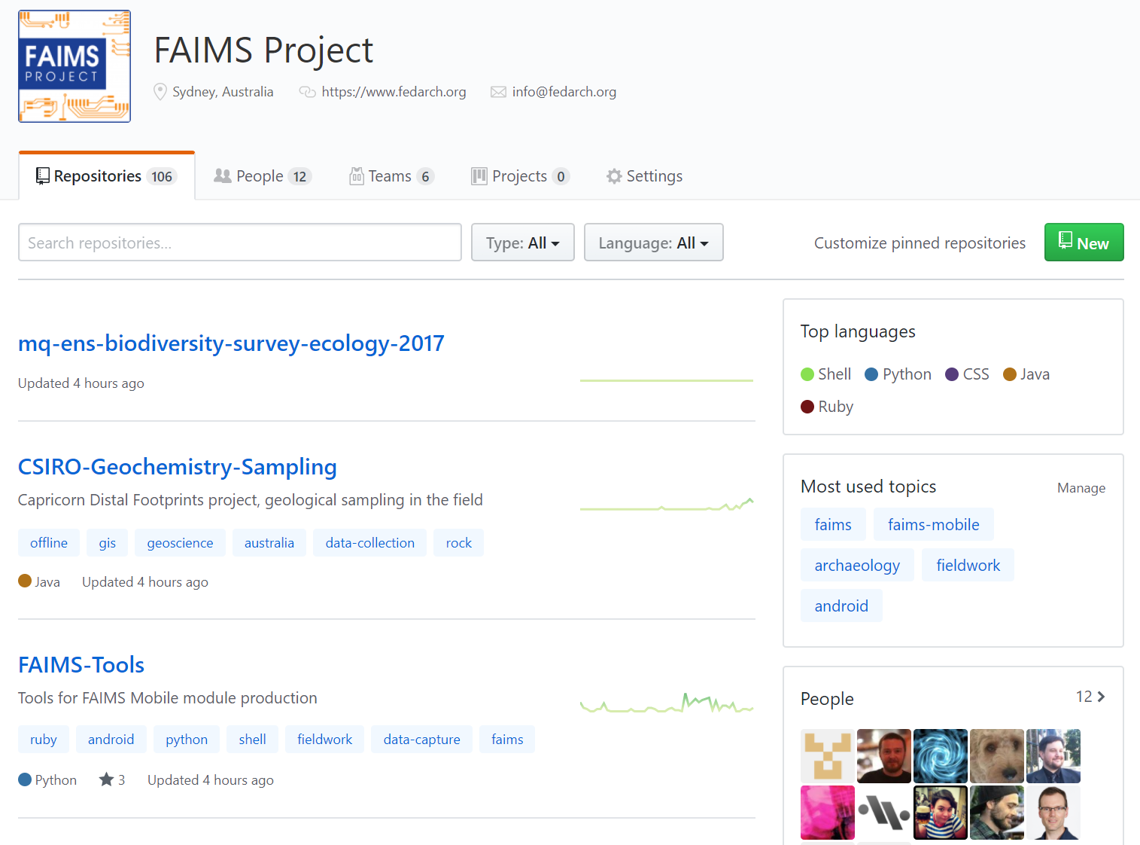
\includegraphics[height=.75\textheight]{figures/FAIMS-generalised.png}
        \caption{FAIMS Mobile customisations (XML files, mostly) on GitHub}
        \label{fig:figure11}
 \end{figure}
\end{frame}

\begin{frame}{Modular and federated}
  Do one thing well.
      \begin{itemize}[label=\textbullet]
        \item Identify other infrastructure in the domain and interoperate with it (via ETLs or APIs).
        \item It is better to divide by data-lifecycle phase rather than data type, since (1) our data is so integrated and (2) field data capture poses unique challenges.
    \end{itemize}
\end{frame}

\begin{frame}{Modularise by data lifecycle phase}
 \begin{figure}[H]
    \centering
        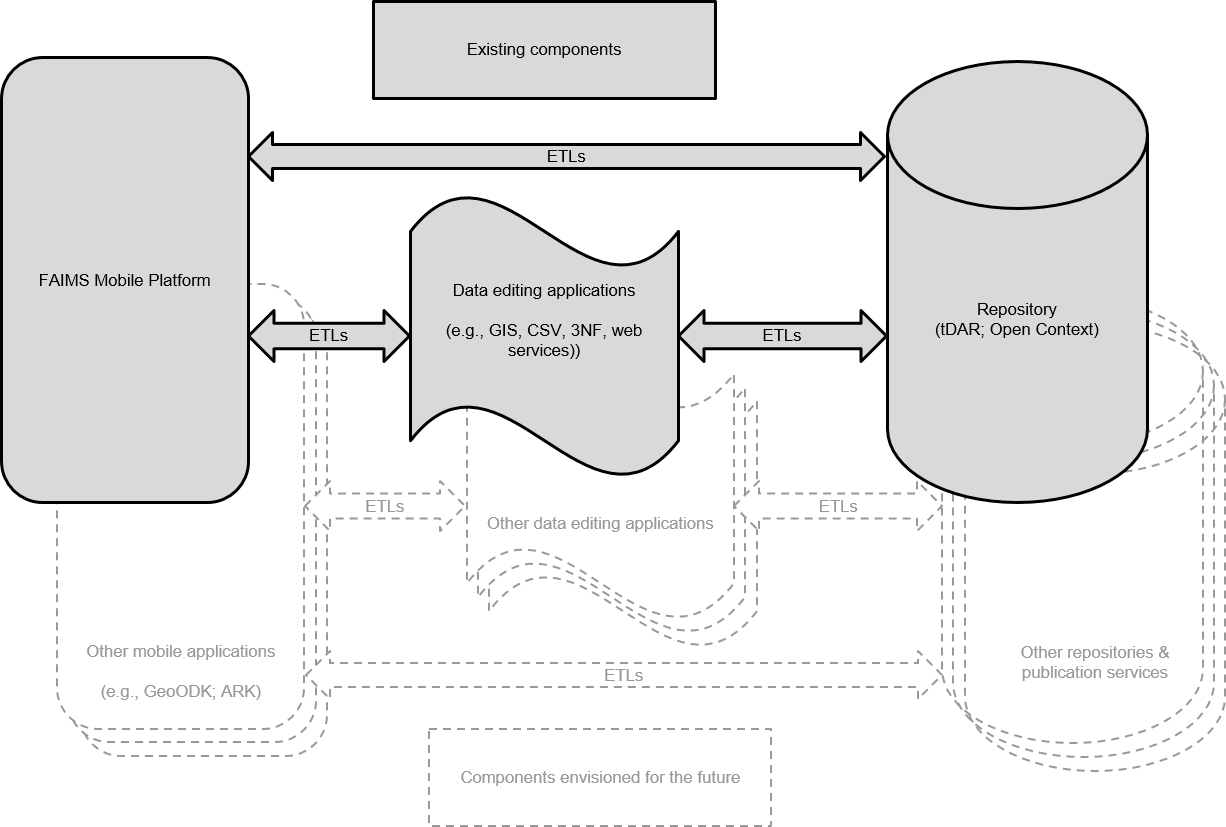
\includegraphics[height=.75\textheight]{figures/FAIMS-federated.png}
        \caption{FAIMS Mobile federation strategy}
        \label{fig:figure13}
 \end{figure}
\end{frame}

\begin{frame}{Open source?}
  Open source has advantages but is difficult to sustain.
      \begin{itemize}[label=\textbullet]
        \item Emerging open research principles strongly prefer OSS as opposed to proprietary ‘black boxes’.
        \item Transparency and reusability (esp. customisation code).
        \item Ability to hand off from one organisation to another (esp. `core' platform code).
        \item Ability to fork code prevents lock-in and mitigates unwelcome decisions by software developers.
        \item BUT OSS business models are hard to scale and rely on occasional injections of grant or institutional funding.
    \end{itemize}
\end{frame}

\begin{frame}{Scope carefully}
  Talk to a wide range of potential users, seeking facts not opinions.
      \begin{itemize}[label=\textbullet]
        \item Don’t ask researchers what they think, ask them what they have done - what software they have adopted and why, and what problems they have expended resources to solve. 
        \item ‘Lean startup’ methodology very useful, based around  testing of ideas through interviews with potential users \cite{Strategyzer_AG2019-uu}.
        \item In our case, we over-invested in mobile GIS and under-invested in usability (especially a GUI for customisation).
    \end{itemize}
\end{frame}

\begin{frame}{Spend on outreach and engagement}
  If you build it they will not come; people can't use technologies they don't know about.
      \begin{itemize}[label=\textbullet]
        \item As per industry standards, dedicate at least 30\% of any information infrastructure budget to outreach and engagement (sales and marketing). 
        \item Typical academic outreach (journal articles, conference presentations, workshops, even booths at major conferences) are not enough.
    \end{itemize}
\end{frame}

\begin{frame}{FAIMS publications}
      \begin{itemize}[label=\textbullet]
        \item \cite{Sobotkova2018-al}
        \item \cite{Ballsun-Stanton2018-zd}
        \item \cite{VanValkenburgh2018-hv}
        \item \cite{sobotkova2016-mx}
        \item \cite{Ross2015-ph} 
        \item \cite{Sobotkova2015-lq}
        \item \cite{Ross2013-hi}
    \end{itemize}
\end{frame}

\begin{multicols}{2}[]
\bibliography{references}
\bibliographystyle{apalike}
\end{multicols}

\section{From current practice to better practice}

\begin{frame}{Challenges and paths forward}
  How do we get from where we are now to where we want to be?
      \begin{itemize}[label=\textbullet]
        \item Understand the evolving expectations of transparent research. 
        \item Look past desktop software (Excel, ARCGIS, Filemaker, Access, etc.).
        \item Rally around emerging research- and domain-specific solutions (even if imperfect).
        \item Overcome `not invented here'; you don't need a bespoke solution.
        \item Budget for `ground-up' transparency (data and code). Up-front costs will be high but offer longer-term payoffs (in costs, time, and quality).
        \item Implement (and budget for) fundamental good practice in data and code management before other technologies.
        \item Improve research design (prioritise approach over methods) \cite{Muthukrishna2019-kt, Hole1973-cy}
    \end{itemize}
\end{frame}
% \bibliographystyle{apalike}

 
% Adding the option 'allowframebreaks' allows the contents of the slide to be expanded in more than one slide.
% The "1" comes from the outer theme"

\section{References}

% \begin{frame}[allowframebreaks]{References}
  
%   \bibliography{references}
%   \bibliographystyle{apalike}
% \end{frame}


\begin{frame}{Thank you!}

%This presentation is available at:
%\texttt{https://osf.io/v5jp7/}

Source code for this presentation is available at: 
\texttt{https://github.com/ saross/Ross-FAIMS-current}.

FAIMS Project software and documentation can be found at:
\texttt{https://github.com/faims}.

This work is licensed under a Creative Commons Attribution 4.0 International License.

\end{frame}



\end{document}
